\documentclass[UTF8]{ctexart}
\usepackage{amsmath}
\usepackage{amssymb}
\usepackage{background}
\usepackage{booktabs}
\usepackage{caption,subcaption}
\usepackage{CJKfntef}
\usepackage{enumitem}
\usepackage{fancyhdr}
\usepackage{float}
\usepackage{fontspec}
%\usepackage{fourier}
\usepackage{geometry}
\usepackage{imakeidx}
\usepackage{makecell}

%\usepackage{tcolorbox}
%\tcbuselibrary{breakable, raster}
%\usepackage{tikz}
%\usetikzlibrary{arrows.meta}
\usepackage{url}
\usepackage{xcolor}

\geometry{a5paper, top=0.1cm, left=1cm, right=1cm, bottom=1cm, footskip=0.6cm, marginparsep=0.1cm}

\setCJKmainfont[BoldFont={汉仪文黑-85W},ItalicFont={方正苏新诗柳楷简体}]{思源宋体 CN}
\setfontfamily\Issue{Century Schoolbook}
\setfontfamily\Genshin{Genshin Teyvat Lingua Franca}
\newCJKfontfamily\TitleFont{思源宋体 CN Heavy}
\newfontfamily\timesnewroman{Times New Roman}
\captionsetup{font=small, labelfont=bf}
\setlist[itemize]{itemsep=0pt, parsep=0pt}

\pagestyle{fancy}
\fancyhf{}
\cfoot{\ttfamily\footnotesize{-\ \thepage\ -}}
%\reversemarginpar

%\CTEXsetup[format = {\centering\bfseries\large}, beforeskip = 3pt, afterskip = 3pt]{section}
\CTEXsetup[format = {\color{cyan!50!black}\bfseries\large}]{subsection}

\makeindex[columns=2, title={名词索引}, columnseprule] % 索引格式

%\newtcolorbox{process}[1]{colback=cyan!10, colframe=cyan!50!black, boxrule=0.5pt, title={#1}, breakable}

\colorlet{darkcyan}{cyan!50!black}
\newcommand\Black[1]{\textcolor[gray]{0.3}{#1}}
\newcommand\Brown[1]{\textcolor[HTML]{998A4E}{#1}}
\newcommand\Emph[1]{\colorbox{green!10}{\textcolor{green!30!black}{#1}}}
\newcommand\Concept[1]{\textcolor{cyan!70!black}{#1}}
\newcommand\Notes[1]{\textcolor{yellow!50!black}{\small #1}}
\newcommand\Example[1]{\textcolor{cyan!70!black}{\small #1}}
\newcommand\means[1]{\textcolor{cyan!70!black}{#1}}



\newcommand\IssueNumber{41}
\newcommand\Date{2024-11-13}
%\newcommand\Contributer{@金光日}
\newcommand\Subject{计算机网络}
%\newcommand\Source{2022 考研 408 第 5 题}


\begin{document}
\backgroundsetup{contents=
\includegraphics{上半示例.png}, center, scale=1, angle=0, opacity=1}
\BgThispage
\begin{center}
%{\scriptsize\Issue \textcolor[HTML]{C8BA83}{\Genshin WEEKLY TIPS}}
\phantom{...}

{\Large\textcolor{brown!40!white}{\makebox[10cm][s]{\Genshin WEEKLY KNOWLEDGE TIPS}}}

\vspace{-2em}

{\Huge\bfseries\TitleFont \Black{知\ 识\ 小\ 料}}


\vspace{-0.1cm}
{\footnotesize \Brown{「电计 2203 班」周常规知识整理共享}}
\end{center}

\vspace{-0.5cm}


\begin{figure}[H]
\hspace{1cm}
\begin{minipage}[t]{0.3\textwidth}
\centering
    \Brown{\Genshin ISSUE}

    \vspace{-0.6cm}
    \Huge \Issue\slshape\bfseries\Black{\IssueNumber}
\end{minipage}
\hfill
\begin{minipage}[t]{0.35\textwidth}
\small
\centering
    \Brown{日期:\Date} \\
%\vspace{-0.1cm}
%    \Brown{贡献者:\Contributer} \\
\vspace{-0.1cm}
    \Brown{学科:\Subject} \\
%\vspace{-0.1cm}
%    \Brown{来源:\Source}
\end{minipage}
\hspace{0.8cm}
\end{figure}

{\color{darkcyan}
本文档用于对《计算机网络》作出简明复习,自顶向下讲述。

互联网究竟是什么样的?从硬件来看,有许多网络边缘和网络核心部件;从软件来看,有许许多多的协议,约定着硬件们通信的方法。

互联网由一个个「网络的网络」相连。数据、报文在网络边缘之间传递,需要考虑多种多样的因素,如延迟、丢包、稳定性……从 1967 年的 ARPANET「阿帕网」问世,网络经过一轮一轮的迭代,逐渐演化成了今天我们看到的模样。
}


\section{应用层}
如今应用层有两种服务模式:C-S模式和 P2P 模式,前者应用居多。我们的电脑与客户端通信,其实是一个个进程与客户端的相关进程通信。这些进程,象征着网络中通信的结点,我们称之为\Concept{「套接字」(socket)}\index{socket(套接字)}。套接字是承应用层、启传输层的一个小层。

怎么定位一个互联网上的网站呢?可以使用 IP 地址,但更常见的做法是使用域名。域名对人类阅读更友好,但计算机不认识它们,所以就有了\Concept{「域名解析协议」(DNS)}\index{DNS(域名解析协议)}。DNS 是将域名与 IP 地址建立关系的映射表。

一个域名通常由多级组成,越靠右级别越高,比如 \url{ys.mihoyo.com} 域名由三级域名 \texttt{ys}、二级域名 \texttt{mihoyo}、一级域名 \texttt{com} 组成。由这些等级,理论上可以把全世界的域名用一棵域名树来管理。DNS 查询域名的 IP 地址有两种方式:递归查询、迭代查询。

管理网页内容的一种协议是\Concept{「超文本传输协议」(HTTP)}\index{HTTP(超文本传输协议)},它使用 TCP 作为下层协议服务。我们通过输入网址访问一个网页的流程通常如下:
\begin{enumerate}[itemsep=0pt,parsep=0pt]
  \item 浏览器分析输入的网址——学名\Concept{「统一资源定位符」(URL)}\index{URL(统一资源定位符)};
  \item 浏览器向 DNS 请求解析出 IP 地址;
  \item DNS 成功解析出对应的 IP 地址;
  \item 浏览器与服务器建立 TCP 连接;
  \item 浏览器发出 HTTP 请求报文——GET 格式;
  \item 服务器发回 HTTP 响应报文;
  \item 释放 TCP 连接;
  \item 浏览器将网站所指文件的内容显示出来。
\end{enumerate}

以上便是应用层的基本知识。

\backgroundsetup{contents=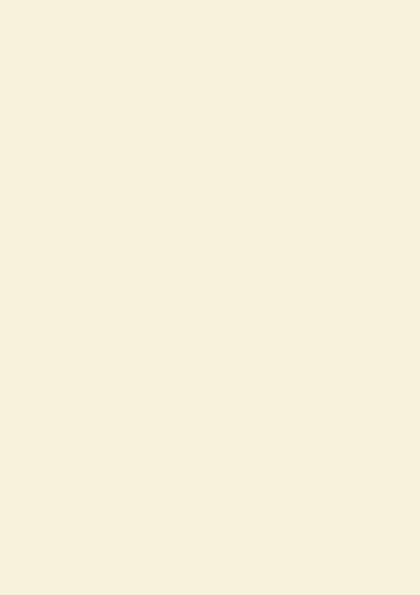
\includegraphics{空白示例.png}, center, scale=1, angle=0, opacity=1}
\BgThispage
\section{传输层}
传输层用于提供端到端的逻辑通信,以 TCP 和 UDP 两个协议主导。报文在这一层将变成「报文段」。

传输层要处理来自应用层不同套接字的数据,并合并下放到网络层,这便是「多路复用」。它还要将从网络层上传的报文段分类上传到不同的套接字,这便是「多路分解」。因而为了区分进程,一个 TCP 套接字用四元组表示:(源 IP 地址,源端口号,目的 IP 地址,目的端口号)。

\subsection{UDP}
接下来是\Concept{「用户数据报协议」(UDP)}\index{UDP(用户数据报协议)}。从总体来说,UDP 无连接,不可靠,不自动重传,全双工通信。但是它相比 TCP 有两个明显优势:
\begin{itemize}[itemsep=0pt,parsep=0pt]
  \item UDP 协议简单方便
  \item UDP 延迟低,速度快
\end{itemize}
因此在一些场合,还是需要使用 UDP 而非 TCP。

UDP 头部有 8 字节,其中的「总长度」包括头部在内($8\sim 65535$ 字节)。由于 UDP 不会理会数据长度到了链路层是否超过 \Concept{「最大传输单元」(MTU)}\index{MTU(最大传输单元)},因此用 UDP 要发合适大小的报文段。

为了让数据传输看起来更可靠,我们引入了\Concept{「可靠数据传输协议」(rdt1.0 $\sim$ 3.0)}\index{rdt(可靠数据传输协议)}。它包含四个接口组:\verb!rdt_send()!、\verb!udt_send()!、\verb!rdt_rcv()!、\verb!deliver_data()!。而 rdt 从 1.0 演化到 3.0 也采取了许多举措使得传输看起来更可靠。
\begin{itemize}[itemsep=0pt,parsep=0pt]
    \item 错误检测与确认应答——rdt2.0
    \item 字节编号与顺序控制——rdt2.1
    \item 丢弃 NAK 只使用 ACK——rdt2.2
    \item 定时重传——rdt3.0
\end{itemize}

\subsection{TCP}
接下来是\Concept{「传输控制协议」(TCP)}\index{TCP(传输控制协议)}。从总体上看,TCP 是全双工通信,比 UDP 多了许多机制,比如三次握手、四次挥手、流量控制、拥塞控制等,相对复杂。

TCP 头部有 20 字节,其中的「总长度」包括头部在内。但需要指明,\Concept{「最大数据长度」(MSS)}\index{MSS(最大数据长度)}\textcolor{red}{不包括}头部长度。

TCP 通信时,伴随着序号和确认号的机制。确认号总是对方下一个报文的起始字节的编号。建立 TCP 通信时,会经过三次握手的过程;断开 TCP 通信时,会经过四次挥手的过程。

TCP 维护一个发送窗口,发送窗口是流量窗口(rwnd)和拥塞窗口(cwnd)的较小者。流量窗口由接收端管理,它标志着发送端最多可发送的数据量,以免接收端一次接收过多的数据。拥塞窗口由发送端管理,它标志着当前受信道拥塞情况最多可发送的数据量,以免导致网络拥堵。拥塞窗口的维护分为「慢开始算法」和「拥塞避免算法」两个算法,遵循加法增大和乘法减小的原则。

以上就是传输层的基本知识。

\section{网络层}
在网络层中,我们研究数据报本身和它转发的方法(数据平面),也研究数据报在整个网络中「导航」的方式(控制平面)。路由器是网络层里几乎最重要的设施。

\subsection{数据平面}
对于一个路由器而言,数据报在其中交换,遵循内存交换、总线交换、互联网络交换等方式,路由器尽力而为地服务。路由器自身的输出端口会控制数据报的流动,存在缓存管理、尾部丢弃、循环调度、同级排队先来先服务等机制。

\Concept{「网际互连协议」(IP)}\index{IP(网际互连协议)}贯穿着网络层的方方面面。IP 强调适应性、简洁性、可操作性,而不保证时效性、可靠性,这是为了适应异构网络。

IPv4 头部有 20 字节,其中的「总长度」包括头部在内。如果一个数据报太大,它便会被分片,这时候的标识、标志、片偏移字段会起作用:标识是组号,标志是 $\mathrm{(0,MF,DF)}$ 三位字段,片偏移是这一段相对第一段相差的字节数除以 8 得到的值。

IPv4 地址采用点分十进制表示法,由 32 位二进制数构成。IPv4 地址分为网络号和主机号。由于 IPv4 地址数量不大,因此人们发明了种种治标但不治本的方法来缓解 IPv4 地址用完的窘境:
\begin{description}[itemsep=0pt,parsep=0pt]
  \item[地址分类] 把 IP 地址分成 A,B,C,D,E 五类,如 A 类地址有8位网络号、24位主机号,等等。人们规定了一些特别的 IP 地址,如全 0 型保留备用,主机号全 1 型分组广播,32 位全 1 型为受限广播、127.0.0.1 为回送地址。
  \item[CIDR] \Concept{「无分类域间路由选择」(CIDR)}\index{CIDR(无分类域间路由选择)}引入了子网掩码的概念,让 IP 地址与子网掩码做与运算得到网络号。使用 CIDR 能将一个网络划分为若干个子网,也可以用于路由表汇聚(按最长前缀匹配),是考试重点。
  \item[NAT] \Concept{「网络地址转换」(NAT)}\index{NAT(网络地址转换)}区分了全局与局部的 IP 地址。外界找内网的主机,只看连接内网侧的路由器对应的全局 IP 地址;而内网的 IP 地址即使与外界的 IP 地址重合也没有影响。
\end{description}

路由表工作的流程是「匹配+行动」(Match+Action)。匹配操作遵循「最长前缀匹配」:如果目标 IP 地址同时满足路由表中的多个地址,那么路由器会取带有最长网络号前缀的那个地址来匹配,取对应地址条目的端口转发——事实上就是「最具体前缀匹配」。行动操作不止是转发操作,而包含了转发、丢弃、修改头部、上报至控制器等若干个操作。比如路由器通常匹配+转发,而防火墙通常匹配+丢弃。这体现了 OpenFlow 流表思想。

然而,IPv4 地址终究不够,我们最终还是得使用 IPv6 地址:它采用了冒分十六进制表示法,由 128 位二进制数构成。如果要混用 IPv4 和 IPv6,那么可以将 IPv6 的全部内容塞进 IPv4 的数据字段中,是为「隧道式转发」。

在连上网时,主机如何获得一个 IP 地址?\Concept{「动态主机配置协议」(DHCP)}\index{DHCP(动态主机配置协议)}这个\textcolor{red}{应用层}协议会给出答案。DHCP 服务器位于路由器中,为路由器连接的所有子网提供服务。一般客户向 DHCP 服务器申请 IP 地址有四个步骤:客户端申请地址、服务器提供地址、客户端请求使用、服务器确认请求。

网络层传输有异常怎么办?\Concept{「网际控制报文协议」(ICMP)}\index{ICMP(网际控制报文协议)}这个\textcolor{red}{网络层}协议会报告它。ICMP 负责报告差错,但不负责处理纠正。ICMP 有两种查询报文:回送请求+回答报文、时间戳请求+回答报文,其中前者正是 \verb!ping! 命令的原理。

\subsection{控制平面}
路由器内部维护路由表和路由算法,其中路由算法对数据报在整个大网络中的「导航」有重要作用。

有以下两种著名的路由算法:
\begin{description}[itemsep=0pt,parsep=0pt]
  \item[链路状态算法(LS)] \index{LS(链路状态算法)}常用的有 Dijkstra 算法。假设 $N'$ 是已确定最短路径的结点集合,初始仅包含起点。在每一轮迭代中,上一个被放入 $N'$ 的结点 $w$ 的最短路径长度 $D(w)$,会更新所有 $D(v)$($\forall v\notin N'$),计算公式:
      \begin{equation*}
            D(v)\gets \min\{D(v),\  D(w)+c_{w,v}\}\text{,对任意} v\notin N'
      \end{equation*}
      此后选取 $D(v)$ 值最小的结点 $v$ 放入 $N'$ 中,一轮迭代完成。这个算法会持续到所有结点都被放进 $N'$ 为止。
  \item[距离向量算法(DV)] \index{DV(距离向量算法)}常用的有 Bellman-Ford 算法。假设 $D_x(y)$ 是从结点 $x$ 到结点 $y$ 的当前最短路径,它会由 $x$ 的所有直接邻居 $v$ 的信息来更新:
      \begin{equation*}
            D_x(y)\gets \min\limits_{v} \{c_{x,v} + D_v(y)\}
      \end{equation*}
      直到所有的 $D_x(y)$ 均不更新才结束。
\end{description}

在大网络中,设有许许多多个\Concept{「自治系统」(AS)}\index{AS(自治系统)},它们可能以国家、省份或城市为单位。这些自治系统之内用\Concept{「内部网关协议」(IGP)}\index{IGP(内部网关协议)}来通信,自治系统之间用\Concept{「外部网关协议」(EGP)}\index{EGP(外部网关协议)}来通信。

基于上述的两种路由算法,我们学习了两种典型的 IGP 协议和一种典型的 EGP 协议。这些协议的对比简表,如表 \ref{tab:对比表} 所示。

\begin{description}[itemsep=0pt,parsep=0pt]
  \item[OSPF] \Concept{「开放最短路优先协议」(OSPF)}\index{OSPF(开放最短路优先协议)}是一种 IGP 协议,用于自治系统之内的通信。它使用链路状态算法(LS)即 Dijkstra 算法更新,是网络层协议,追求代价最小。在这里,每个路由器都有完整的拓扑结构;每个路由器都会直接通过 IP 数据报将\textcolor{red}{相邻路由器的链路状态},通告到整个 AS 中的\textcolor{red}{所有}路由器。
  \item[RIP] \Concept{「路由信息协议」(RIP)}\index{RIP(路由信息协议)}也是一种 IGP 协议,用于自治系统之内的通信。它使用距离向量算法(DV)更新,基于 UDP 传输,是应用层协议,追求跳数最少。由于距离为 16 表示不可达,因此 RIP 允许一条路径最多有 15 个路由器,只适用于小型网络。每个路由器会将自己的路由表发送到相邻的路由器。
  \item[BGP] \Concept{「边界网关协议」(BGP)}\index{BGP(边界网关协议)}是一种 EGP 协议,用于自治系统与自治系统之间的通信。BGP 是\textcolor{red}{应用层}协议,基于 \textcolor{red}{TCP} 传输,用路径向量法更新,追求一条能到达的比较好的路径,不追求最佳。每个 AS 中都有「BGP发言人」,每个 BGP 发言人会将路由信息发送到一些相邻的 BGP 发言人;这些路由信息在连接开始时是整个路由表,在连接过程中是有变化的部分。

      此外,在内部 iBGP 中,路由器使用「烫手的土豆」传输法:路由器总是向域内成本最低的路由器传输,不管域外成本有多高。
\end{description}

\begin{table}[htb]
\small
  \centering
  \begin{tabular}{ccccccc}
  \toprule
    协议 & 内/外 & 层级 & 传输基础 & 追求 & 交换信息 & 向谁交换 \\
  \midrule
    OSPF & 内 & 网络层 & IP & 代价少 & 相邻路由器链路状态 & AS 中所有路由器\\
    RIP & 内 & 应用层 & UDP & 跳数少 & 自身路由表 & 相邻路由器 \\
    BGP & 外 & 应用层 & TCP & 比较好 & 路由表,或变化部分 & BGP发言人\\
  \bottomrule
  \end{tabular}
  \caption{三种路由协议对比简表}\label{tab:对比表}
\end{table}

那么,各个路由器的路由表和路由算法靠什么控制呢?我们称之为\Concept{「软件定义网络」(SDN)}\index{SDN(软件定义网络)}。SDN 是一种新型的网络控制架构,通过控制端,远程向每个路由器安装路由表和路由算法。这个控制的过程和路由算法归属于控制平面,而路由表归属于数据平面,这样就实现了数据平面与控制平面的分离。在 SDN 模式下,路由器的工作就变得很单纯,即收到分组、查找转发表、转发分组。

\textcolor{cyan}{(\CJKsout{控制平面是这样的。路由器只需要收到并转发分组就可以,可是 SDN 和控制平面要考虑的事情就很多了。})}

SDN 控制器分三层:底层与设备通信,中层统计流表等数据,顶层是各种应用接口。SDN 使用「北向接口」(也就是顶层)与网络控制程序软件交互,使用「南向接口」(也就是底层)与路由器设备交互。SDN 的一个底层 API 是 OpenFlow。如果有设备故障,则会经历如下过程:底层接口获取信息——中层更新状态信息——顶层计算新路由表——中层发起新的控制——底层对设备安装新表。

%\begin{enumerate}[itemsep=0pt,parsep=0pt]
%    \item 设备故障,OpenFlow底层接口通知中层控制器;
%    \item 中层更新链路状态信息,上传至顶层控制应用程序;
%    \item 顶层根据中层提供的信息,计算新的路由表;
%    \item 中层接收顶层的计算结果,向底层发起控制;
%    \item 底层对设备安装新路由表。
%\end{enumerate}


为了实现前后端分离,引入了「表现层状态转移」(RESTful)结构。这种结构可以使资源集中存放,同时使用户能够像访问自己电脑的文件一样访问海量的资源。

以上内容,便是网络层的基础知识。

\section{(有线)链路层、局域网}
链路层的作用,是将「帧」从一处传递到另一处。在链路中传输可能有错误,常用的检测手段有奇偶校验、CRC 循环冗余校验。在电脑里,有一个称为「网络接口卡」(NIC)的小部件,用于计算机与局域网的通信。

\subsection{多路访问与 CSMA/CD}
最初的以太网用广播的方式通信。但如果一个结点同时接收到多个信号,就会发生碰撞。为了避免碰撞,人们发明了时分、频分多路复用等方式。要随机访问,可以用 ALOHA 方式来通信。然而,ALOHA 的效率很低,因此又发明了新的方式 CSMA/CD 和 CSMA/CA。

在以太网中,实行\Concept{「载波侦听多路访问·冲突检测」(CSMA/CD)}\index{CSMA/CD(载波侦听多路访问·冲突检测)}的方式。这是一种半双工(双向交替通信)的方式,其主要内涵是「先听后发,边听边发;冲突停止,延迟重发」。当发送方检测到冲突后,就发送噪声帧,让链路中的所有结点都能感知到冲突。随后取随机延迟时间等待后重新发送。
\begin{itemize}[itemsep=0pt,parsep=0pt]
  \item 最短有效帧长是 512bit(64B),小于这个长度的帧会被视为无效(如 48bit 的噪声帧)。
  \item 争用期 $2\tau$ 是 512bit 所需时间(对于 10Mb/s 以太网取 $\mathrm{51.2\mu s}$),若经过争用期的时间后没有冲突,即可确定后续不会发生冲突。
  \item 帧间最小间隔为 96bit(12B)所需时间(对于 10Mb/s 以太网取 $\mathrm{9.6\mu s}$),从检测空闲到发送数据要经历一个间隔,以刷新缓存。
  \item 随机延迟:遵循\Concept{「截断二进制指数退避算法」}\index{截断二进制指数退避算法}:先确定基本退避时间为争用期 $2\tau$。设 $n(\leqslant 10)$ 为碰撞次数;指定倍数 $k = \mathrm{rand}\{0,1,2,\dots, 2^n-1\}$,则设定延迟时间为 $2k\tau$。如果重传次数超过 10 次,则 $n$ 设定为 10;如果重传次数超过 16 次,则丢弃帧并向高层报告。
\end{itemize}

\subsection{MAC 地址}
每个设备皆有MAC地址。对于一台设备,IP地址犹如家庭住址,可变;而MAC地址犹如身份证号,不可变。MAC 地址由 48 位二进制数构成。

就像 DNS 能从域名解析出 IP 地址一样,\Concept{「地址解析协议」(ARP)}\index{ARP(地址解析协议)}能从 IP 地址解析出 MAC 地址。ARP 表的每个条目记录的是三元组 $(\mathrm{IP,MAC},TTL)$。ARP 的查询是广播帧,响应是标准帧;因此在查询时,广播域中的每个主机都能收到帧,但只有特定的几个主机会接受帧,并发送响应帧。

ARP 表只服务于所在的子网,因此数据从一个子网到另一个子网传输时,源和目标 IP 地址不变(即全局的起点和终点),但是 MAC 地址会辗转变化(即子网内的起点和终点)。

\subsection{以太网 802.3 协议}
决定以太网性能的三要素:网络拓扑、传输介质、介质访问控制方法。以太网拓扑有总线网、星形网、环形网,其中后两种今天更常见一些。

以太网\Concept{802.3 协议}\index{802.3(以太网协议)}的一帧有相应格式,数据字段长度为 $46\sim 1500$ 字节。上限为 1500 正是「最大传输单元」(MTU)限制的长度。下限为 46 是为了使最小长度达到最短有效帧长,带上头尾总长 $46+18=64$ 字节,防止被丢弃。由此可见,如果数据字段本身不足 46 字节,则需要填补到 46 字节。

以太网标准 802.3 还约定了链路层和物理层的格式,其中约定了物理层的传输介质,如 100BASE-TX, -T2, -T4 等 T 开头的表示介质为双绞线,100BASE-FX, -SX, -BX 等 X 结尾的表示介质为光纤。802.11 标准约定的是无线网络的标准。

\subsection{扩展以太网}
扩展以太网有\Concept{共享式局域网}\index{共享式局域网}和\Concept{交换式局域网}\index{交换式局域网},前者从物理层扩展,用到中继器、集线器;后者从链路层扩展,用到网桥、交换机。

在共享的以太网中,存在着\Concept{「冲突域」}\index{冲突域}和\Concept{「广播域」}\index{广播域}。顾名思义,冲突域(也叫碰撞域)是可以发生碰撞的设备集合,广播域是单个广播消息能传输到的范围。

\begin{itemize}[itemsep=0pt,parsep=0pt]
  \item 「中继器」工作在物理层,用于信号的放大和再生。距离不能太远,且链接的网段速率相同。
  \item 「集线器」工作在物理层,相当于多接口的中继器,可以将多个结点连成一个共享式局域网。
  \item 「网桥」工作在链路层,可互联不同物理层、不同网段速率的局域网。
  \item 「交换机」工作在链路层,相当于多端口的网桥,是交换式局域网的核心设备,通常在全双工方式工作,受硬件控制。
  \item 通过交换机还可以实现「虚拟局域网」(VLAN),可以实现流量隔离,也允许多个交换机通过干线连接(trunk)共享一个VLAN。
  \item 「路由器」工作在网络层,受软件控制(SDN),按路由算法转发数据报。
\end{itemize}

交换机有自学习机制。在有帧到达交换机时,若无目标 MAC 地址匹配则以「洪泛法」广播转发,并记下源地址对应端口的条目;若有目标MAC地址记录则按对应的端口转发,其中当目标地址即为源地址时遣返该帧。

关于是否隔绝冲突域和广播域的设备,总结如下:
\begin{itemize}[itemsep=0pt,parsep=0pt]
  \item 中继器、集线器:不隔绝冲突域,也不隔绝广播域;
  \item 网桥、交换机:隔绝冲突域,但不隔绝广播域;
  \item VLAN、路由器:既隔绝冲突域,也隔绝广播域。
\end{itemize}

\section{无线网络}
无线网络相比有线网络衰减更明显,干扰更强,沿多路传播。无线网络一般有两种分类方法,即分为有基础设施/无基础设施、单跳/多跳,例如 WiFi、蜂窝数据是有基础设施的单跳无线网络,蓝牙是无基础设施的单跳无线网络。

无线网络使用 \Concept{802.11 协议}\index{802.11(无线网络协议)} 这个协议家族,有\Concept{「接入点」(AP)}\index{AP(接入点)}(也就是基站)和\Concept{「基本服务集」(BSS)}\index{BSS(基本服务集)},我们常说的「主机接入网络」就是一个基本服务集的主机访问一个接入点。在接入时,主机需要扫描与听取诸多 AP 的名称(SSID)和MAC地址,随后选择一个 AP 访问。于是经过认证,经由 DHCP 协议后就可以获得一个 IP 地址。这一扫描过程分为「被动扫描」和「主动扫描」两种方式。

\subsection{多路访问与 CSMA/CA}
就像有线网络一样,无线网络也需要多路接入。然而,相比 CSMA/CD(冲突检测),由于信号衰减大导致的噪声帧检测不到,加上「隐蔽站」问题(一次冲突并非每个设备都能检测到),因此改用\Concept{「载波侦听多路访问·冲突避免」(CSMA/CA)}\index{CSMA/CA(载波侦听多路访问·冲突避免)}方式。

在 802.11 协议下,对于发送端:\textcolor{cyan}{(注:$\mathrm{SIFS<DIFS}$)}
\begin{enumerate}[itemsep=0pt,parsep=0pt]
  \item 若信道闲,则经过一个 DIFS(分布式帧间间隔)后发整个帧。
  \item 若信道忙,则随机后退,启用倒计时:忙时暂停,闲时计时,时间用尽则重发整个帧,等ACK。
  \item 若没收到ACK则随机后退,转第2步;若收到ACK则传输成功。
  \item 若要传输更多的帧,则同样随机后退,转第2步。
\end{enumerate}
对于接收端,如果收到帧就在一个 SIFS(短帧间间隔)后返回ACK。

还有一种方法可以解决「隐蔽站」问题,那就是采取「信道预约制」,通过发送 RTS 和 CTS 信号来预约信道,避免冲突。通常用于发送较长的帧。

\subsection{无线网 802.11 协议}
802.11 一帧有相应格式,数据字段长度为 $0\sim 2312$ 字节。下限为 0 是因为不需要冲突检测,不需要判断最短有效帧长。

一帧有三个地址字段,分别表示目的MAC地址、源MAC地址、接收端MAC地址,其中接收端MAC地址表示负责处理这一帧的路由器等设备的地址。一个帧从 802.11 基本服务集(BSS)的一个主机中发出,从主机到接入点(AP)的这一段路途遵循无线的 802.11 协议,从 AP 到 BSS 之外的路由器的这一段路途遵循有线的 802.3 协议。这两个协议的帧格式地址字段的数量和含义均不同。

以上就是链路层与有线、无线局域网的基础知识。

\newpage
\backgroundsetup{contents=
\includegraphics{下半示例.png}, center, scale=1, angle=0, opacity=1}
\BgThispage
\printindex


\end{document} 